\section{Mathematical formulation of SHE}\label{Section2}

This section is devoted to the mathematical formulation of the SHE problem. In what follows, with the notation $\mathcal U$ we will always refer to a finite set of real numbers, contained in the interval $[-1,1]$
\begin{align}\label{eq:Udef}
	\mathcal U = \{u_\ell\}_{\ell=1}^L\subset [-1,1],
\end{align}
with cardinality $|\mathcal U| = L$. 

In broad terms, our objective is to design a piece-wise constant function $u(\tau):[0,2\pi)\to\mathcal U$ such that some of its lower-order Fourier coefficients take specific values determined a priori. 

Due to the application in power converters, we will focus here on functions with \textit{half-wave symmetry}, i.e. 
\begin{align*}
	u(\tau + \pi) = -u(\tau)\quad \mbox{for all}\; \tau \in [0,\pi).
\end{align*}
In this way, $u$ is fully determined by its values in the interval $[0,\pi)$ and its Fourier series only involves the odd terms, thus taking the form
\begin{equation}
	u(\tau ) = \sum_{\underset{i\, odd}{i \in \mathbb{N}}} a_i \cos(i\tau)+ \sum_{\underset{j\, odd}{j \in \mathbb{N}}}  b_j \sin(j \tau), 
\end{equation}
where the coefficients $a_i$ and $b_j$ are given by
\begin{equation} \label{eq:an}
	\begin{aligned}
		a_i = \frac{2}{\pi} \int_0^\pi u(\tau ) \cos(i \tau)\,d\tau, 
		\\
		b_j = \frac{2}{\pi} \int_0^\pi u(\tau)  \sin(j \tau)\,d\tau.
	\end{aligned}
\end{equation}
Because of this half-wave symmetry, in what follows, we will always work with the restriction $u|_{[0,\pi)}$ which, with some abuse of notation, we shall still denote by $u$. We can then give a general formulation of the SHE problem as follows:
\newline
\begin{problem}[SHE]\label{SHEp}
Let $\mathcal{E} _a $ and $\mathcal{E} _b $ be two sets of odd numbers with cardinalities $|\mathcal{E}_a| = N_a $ and $ |\mathcal{E} _b| = N_b$, respectively, and $\mathcal{U}$ be defined as in \eqref{eq:Udef}. Given the vectors $\bm{a}_T \in \mathbb{R}^{N_a}$ and $\bm{b}_T \in \mathbb{R}^{N_b} $, we look for a piece-wise constant function $u: [0,\pi)\to\mathcal{U}$ such that 
\begin{gather}
	\notag a_i = (\bm{a}_T)_i, \quad\textrm{ for all } i \in \mathcal{E}_a,
	\\
	\notag b_j = (\bm {b}_T)_j, \quad\textrm{ for all } j \in \mathcal{E}_b,
\end{gather}
with $\{a_i\}_{i\in\mathcal E_a}$ and $\{b_j\}_{j\in\mathcal E_b}$ given by \eqref{eq:an}.
\end{problem} 
 
Fig. \ref{fig:exampleSHE} shows an example of a function $u$ solution of the SHE problem. 
 
\begin{figure}
	\centering
	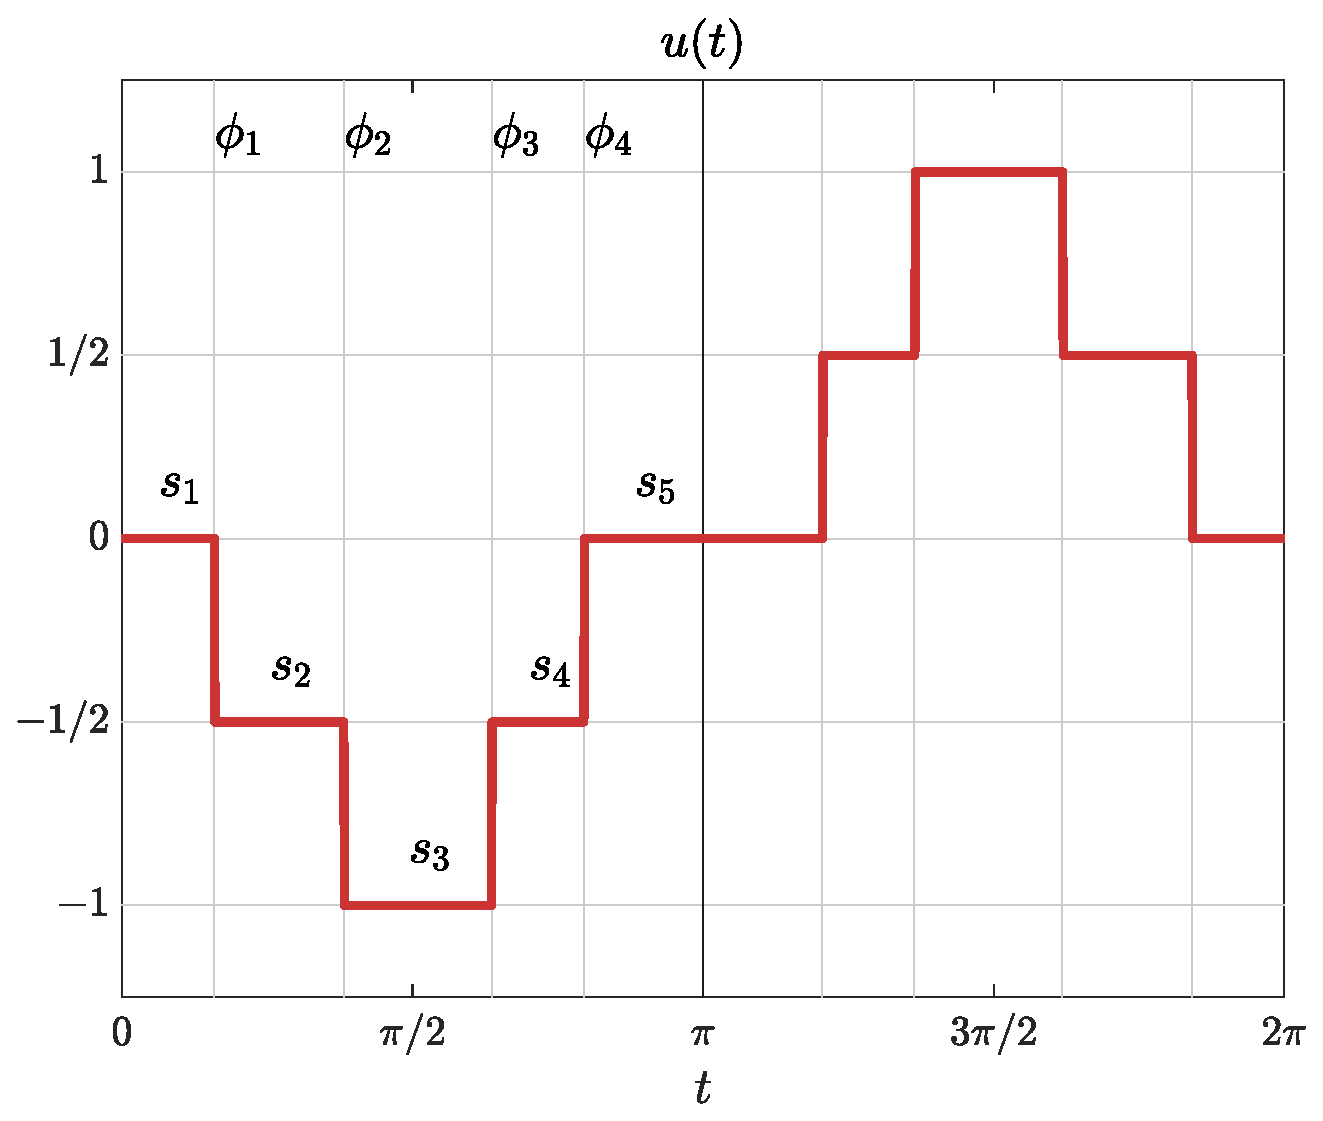
\includegraphics[scale=0.35]{img/fig01.eps} 
	\caption{Possible solution of Problem \ref{SHEp}, where we considered that $\mathcal{U} = \{-1/3, -2/3, 0, 1/3, 2/3, 1\}$. We show the switching angles $\bm{\phi}$ and the waveform $\mathcal{S}$ (see Definitions \ref{def:waveform} and \ref{def:switchingAngles}).}\label{fig:exampleSHE}
\end{figure}

As we anticipated in Section \ref{Section1}, the control signal $u$ is fully characterized by its waveform and the switching angles, to which we now give a precise definition.
\newline
\begin{definition}[Wave-form]\label{def:waveform}
Given the finite set $\mathcal U$ defined in \eqref{eq:Udef} and $M\in\mathbb{N}$, we will call a waveform any possible $(M+1)$-tuple $\mathcal S = (s_m)_{m=0}^{M+1}$ with $s_m\in \mathcal U$ for all $m=0,\ldots,M+1$.
\end{definition}
 
\begin{definition}[Switching angles]\label{def:switchingAngles}
Given the finite set $\mathcal U$ defined in \eqref{eq:Udef}, $M\in\mathbb{N}$ and a piece-wise constant function $u:[0,\pi) \rightarrow \mathcal{U}$, we shall refer as switching angles $\bm{\phi} = \{\phi_m\}_{m=0}^{M+1}\subset[0,\pi]$, with $\phi_0 = 0$ and $\phi_{M+1} = \pi$, to the points in the domain $[0,\pi)$ where $u$ changes its value. 
\end{definition}

In view of the above definitions, we can provide the following explicit expression for $u$:
\begin{align}\label{eq:uExpl}
	&u = \sum_{m=0}^{M+1} s_m\chi_{[\phi_m,\phi_{m+1}]}
	\\
	&s_m\in\mathcal S, \;\phi_m\in{\bm{\phi}}, \quad \mbox{for all } m=0,\ldots,M+1, \notag 
\end{align}
where we denoted by $\chi_{[\phi_m,\phi_{m+1}]}$ the characteristic function of the interval $[\phi_m,\phi_{m+1}]$.

Besides, taking into account \eqref{eq:uExpl}, a direct computation yields that the Fourier coefficients \eqref{eq:an} are given by
\begin{align*}
	& a_i = a_i(\bm{\phi}) =  \frac{2}{i\pi} \sum_{k=1}^{M+1} s_k \Big[\sin(i\phi_k) -\sin(i\phi_{k-1})\Big]
	\\
	& b_j = b_j(\bm{\phi}) = \frac{2}{j\pi} \sum_{k=1}^{M+1} s_k \Big[\cos(j\phi_{k-1}) -\cos(j\phi_{k})\Big]
\end{align*}
Given a waveform $\mathcal S$, Problem \ref{SHEp} then reduces to find the switching locations $\bm{\phi}$ (see \cite{Yang2015,Konstantinou2010,Sun1996}). This can be cast as a minimization problem in the variables $\{\phi_m\}_{m=0}^{M+1}$, where the cost functional is the Euclidean distance between the obtained Fourier coefficients $\{a_i(\bm{\phi}),b_j(\bm{\phi})\}$ and the targets $(\bm{a},\bm{b})\in \mathbb{R}^{N_a}\times \mathbb{R}^{N_b}$.
\newline
\begin{problem}[Optimization for SHE]
Given a waveform $\mathcal S$ and a step function $u$ in the form \eqref{eq:uExpl}, we look for the switching angles $\bm{\phi}$ by means of the following minimization problem:
\begin{align}
	&\min_{\bm{\phi} \in [0,\pi]^{M}} \left(\sum_{i\in\mathcal{E}_a} \|a_T^i - a_i(\bm{\phi})\|^2 + \sum_{j\in \mathcal{E}_b} \|b_T^j - b_j(\bm{\phi})\|^2\right)\notag 
	\\[10pt]
	&\mbox{subject to: } 0 = \phi_0 <\phi_1 < \ldots < \phi_{M} < \phi_{M+1} = \pi \notag 
	\\
\end{align}
\end{problem}

Since the cardinality of $\mathcal S$ is not known a priori, meaning that we do not know how many switches will be necessary to reach the desired values of the Fourier coefficients, a common approach to solve the SHE problem consists in fixing the number of changes and generating all the possible combinations of elements of $\mathcal S$, to later solve an optimization problem for each one of them. Nevertheless, taking into account that the number of possible tuples $\mathcal S$ is given by $|\mathcal{U}|^{|\mathcal S|}$, it is evident that the complexity of the above approach increases rapidly.
%
This problem has been studied in \cite{Yang2015} where, through appropriate algebraic transformations, the authors are able to convert the SHE problem into a polynomial system whose solutions' set contains all the possible waveforms for a given set $\mathcal{U}$ and number of elements in the sequence $\mathcal S$ which, however, is predetermined. 
%

On the other hand, we shall also mention that the SHE methodology has been developed to provide in real-time different target Fourier coefficients con with a $KHz$ latency. 
%
This makes impossible to find real-time solutions by optimization, making then necessary to pre-determine solutions that can later be interpolated.
%
Nevertheless, it is well-known that, fixed a sequence $S$, the continuity of the switching locations with respect to a continuous variation of the target Fourier coefficients may be quite cumbersome. 
%
In the majority of the cases, it is impossible to find a continuous solution in a large interval, an it is necessary to change the waveform $S$ while moving across different solution regions (\cite{Yang2015,Yang2017}). This makes difficult the interpolation of solutions and their finding.

In this document, we will present the SHE problem as an optimal control one, where the optimization variable is the signal $u(\tau)$ defined in the entire interval $[0,\pi)$. 
%
In particular, we will describe how the Fourier coefficients of the function $u(\tau)$ can be seen as the final state of a system controlled by $u (\tau)$. Hence, the optimization is performed among all the possible functions that satisfy $|u(\tau)|<1 $ and can control the final state at the desired Fourier coefficients. Then we will show how to design a control problem so that the solution is a step function.

In this way, we can reformulate Problem \ref{SHEp} as follows.
\newline
In this formulation, the SHE problem converts in a minimization problem with restrictions which can be solved by well-known techniques. Since the problem has several minimizers, we shall solve it employing global optimizers. Furthermore, since the choice of the waveform is arbitrary, we shall proceed in the same way for each possible waveform. 

{\color{red}{
    Tengo que enlazar estas sección con la formulacion de control óptimo.
}}